\chapter{Ensemble grancanonico}
Si consideri un sistema $A$ non isolato e aperto, immerso in un ambiente $B$ molto più grande che funge da bagno termico e chimico, come mostrato in figura \ref{fig: sistema generico (grancanonico)}. In questo sistema, l'equilibrio viene sempre raggiunto alla temperatura $T$ e al potenziale chimico $\mu$ dell'ambiente $B$.
\begin{figure}[h]
    \centering
    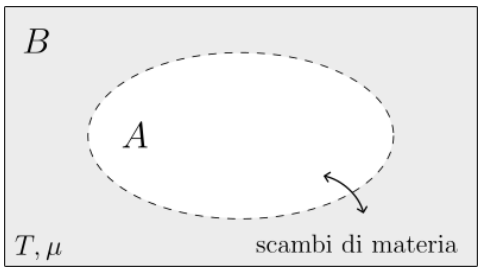
\includegraphics[width=0.4\linewidth]{Immagini/sistema generico (grancanonico).png}
    \caption{sistema generico per l'ensemble grancanonico.}
    \label{fig: sistema generico (grancanonico)}
\end{figure}
Per determinare la distribuzione di probabilità del sistema $A$ all'equilibrio si procede con il massimizzare il funzionale di entropia di Gibbs \eqref{eq: definizione entropia Gibbs} tenendo conto dei seguenti vincoli:
\begin{enumerate}
    \item la probabilità è normalizzata da $\nsum_\nu P(\nu) = 1$;
    \item l'energia dei microstati può fluttuare, ma l'energia media va fissata ad un valore $E$ che, nel limite termodinamico, coincide con l'energia termodinamica, ossia $\vmedio{E} = \nsum_\nu P(\nu)E(\nu) \equiv E$;
    \item il numero di particelle può fluttuare, ma il valor medio va fissato ad un valore $N$ che rappresenta il valore termodinamico di $N$, ossia $\vmedio{N} = \nsum_\nu P(\nu)N(\nu) \equiv N$. 
\end{enumerate}
In modo analogo a quanto fatto per gli ensemble microcanonico e canonico, si introduce per ogni vincolo un moltiplicatore di Lagrange e si massimizza il funzionale di entropia dato da
\begin{equation}
    \begin{split}
        \tilde{\SG}[P] &= \SG[P] + \alpha_0\bigg(\nsum_\nu P(\nu) - 1\bigg) + \alpha_E\bigg(\nsum_\nu P(\nu)E(\nu) - E\bigg) \\
        &+ \alpha_N\bigg(\nsum_\nu P(\nu)N(\nu) - N\bigg)
    \end{split}
\end{equation}
imponendo $\delta\tilde{\SG}[P] = 0$, ossia
\begin{multline}
     \delta\bigg[-k\nsum_\nu P(\nu)\log{P(\nu)} + \alpha_0\bigg(\nsum_\nu P(\nu) - 1\bigg) + \\
     + \alpha_E\bigg(\nsum_\nu P(\nu)E(\nu) - E\bigg) + \alpha_N\bigg(\nsum_\nu P(\nu)N(\nu) - N\bigg)\bigg] = 0.
\end{multline}
Rispetto a variazioni arbitrarie $\delta P(\nu)$ si ha
\begin{equation}
    \nsum_\nu\delta P(\nu)[-k\log{P(\nu)} - k + \alpha_0 + \alpha_EE(\nu) + \alpha_NN(\nu)] = 0,
\end{equation}
da cui, ponendo il termine in parentesi quadra tra parentesi a zero, si ottiene
\begin{equation}
    P(\nu) = \exp{\bigg(-1 + \frac{\alpha_0}{k}\bigg)}\exp{\bigg(\frac{\alpha_E}{k}E(\nu) + \frac{\alpha_E}{k}N(\nu)\bigg)}.
\end{equation}
Imponendo adesso il primo vincolo e ponendo $\exp{(-1 + \alpha_0/k)} \equiv 1/Q$, viene fissato $\alpha_0$ e si ha
\begin{equation}
    \nsum_\nu P(\nu) = \frac{1}{Q}\nsum_\nu \exp{\bigg(\frac{\alpha_E}{k}E(\nu) + \frac{\alpha_E}{k}N(\nu)\bigg)},
\end{equation}
da cui 
\begin{equation}
    Q = \nsum_\nu \exp{\bigg(\frac{\alpha_E}{k}E(\nu) + \frac{\alpha_E}{k}N(\nu)\bigg)},
\end{equation}
mentre il funzionale di entropia diventa
\begin{equation}
    \SG[P] = -k\nsum_\nu P(\nu) \log{P(\nu)} = -k \nsum_\nu P(\nu)\bigg[\frac{\alpha_E}{k}E(\nu) + \frac{\alpha_N}{k}N(\nu) - \log{Q}\bigg].
\end{equation}
Imponendo il secondo e il terzo vincolo, si deduce che $\vmedio{E}$ e $\vmedio{N}$ vanno interpretate come l'energia e il numero di componenti termodinamici 
\begin{equation}
\label{eq: entropia di Gibbs (grancanonico)}
    \SG[P] = -\alpha_E\vmedio{E} - \alpha_N\vmedio{N} + k\log{Q},
\end{equation}
per cui devono valere le equazioni di stato termica e chimica \eqref{eq: equazioni di stato da S} date da
\begin{equation}
\label{eq: equazioni di stato grancanonico}
    \frac{\p S}{\p E}\bigg|_{V,N} = \frac{1}{T} = -\alpha_E,\quad \frac{\p S}{\p N}\bigg|_{E,V} = -\frac{\mu}{T} = -\alpha_N.
\end{equation}
In definitiva, si trova che 
\begin{equation}
    P(\nu) = \frac{1}{Q}\exp{\bigg(-\frac{1}{kT}E(\nu) + \frac{\mu}{kT}N(\nu)\bigg)} = \frac{1}{Q}e^{-\beta[E(\nu) - \mu N(\nu)]},
\end{equation}
dove $Q$ è la funzione di partizione grancanonica
\begin{equation}
\label{eq: funzione di partizione grancanonica}
    Q = \nsum_\nu e^{-\beta[E(\nu) - \mu N(\nu)]}.
\end{equation}
Si ricorda che $\mu$ è l'energia interna termodinamica associata ad ogni singolo componente, quindi solo per il fatto di avere $N$ componenti nel sistema, si ha un certo costo energetico $N\mu$ contenuto nell'energia termodinamica interna. La probabilità grancanonica distribuisce esponenzialmente gli stati in base alla differenza tra $E(\nu)$ e l'energia dovuta al potenziale chimico $\mu N$, quindi
\begin{equation}
    P(\nu) \propto e^{-\beta[E(\nu) - \mu N(\nu)]}.
\end{equation}
Inoltre, risulta spesso conveniente utlizzare la fugacità $z$ che permette di passare dalla coppia di variabili intensive indipendenti $(T,\mu)$ alla coppia di variabili $(T,z)$ 
\begin{equation}
    z \equiv e^{\beta\mu},
\end{equation}
legando il costo di aggiungere e togliere particelle alla scala di energia termica. In questi termini si hanno
\begin{equation}
    P(\nu) = \frac{1}{Q}z^{N(\nu)}e^{-\beta E(\nu)},\quad Q = \nsum_\nu z^{N(\nu)}e^{-\beta E(\nu)}.
\end{equation}
Sostituendo le equazioni di stato \eqref{eq: equazioni di stato grancanonico} nella \eqref{eq: entropia di Gibbs (grancanonico)} si ha
\begin{equation}
    S = \frac{E}{T} - \frac{\mu N}{T} + k\log{Q},
\end{equation}
da cui, moltiplicando per $T$ e riarrangiando i termini, si ottiene l'espressione del potenziale grancanonico 
\begin{equation}
    \varpi(T,V,\mu) = -kT\log{Q(T,V,\mu)} = - \frac{1}{\beta} \log{Q(T,V,\mu)},
\end{equation}
punto di partenza per determinare la termodinamica dell'ensemble grancanonico. Pertanto la funzione di partizione grancanonica $Q$ si può esprimere in funzione di $\varpi$ come
\begin{equation}
    Q(T,V,\mu) = e^{-\beta\varpi(T,V,\mu)}.
\end{equation}
Per quanto riguarda l'energia interna, questa è data da
\begin{equation}
    \begin{split}
        \vmedio{E} = \varpi + TS +\mu N &= \varpi + \beta\frac{\p\varpi}{\p\beta}\bigg|_{V,\mu} - \mu\frac{\p\varpi}{\p\mu}\bigg|_{T,V} \\
        &= \frac{\p}{\p\beta}(\beta\varpi)\bigg|_{V,\mu} - \mu\frac{\p\varpi}{\p\mu}\bigg|_{T,V};
    \end{split}
\end{equation}
invece, in termini della fugacità, si può esprimere $\vmedio{N}$ come
\begin{equation}
\label{eq: numero medio N (grancanonico)}
    \begin{split}
        \vmedio{N} = \frac{1}{Q}\nsum_\nu N(\nu)z^{N(\nu)}e^{-\beta E(\nu)} = \frac{z}{Q}\frac{\p Q}{\p z}\bigg|_{T,V} 
        &= z\frac{\p\ln{Q}}{\p z}\bigg|_{T,V} \\ 
        &= -\beta z\frac{\p\varpi}{\p z}\bigg|_{T,V}.
    \end{split}
\end{equation}
La densità è definita come l'inverso del volume per particella $v$, quindi 
\begin{equation}
    \frac{1}{v} = \frac{N}{V} = -\frac{\beta z}{V}\frac{\p\varpi}{\p z}\bigg|_{T,V}.
\end{equation}
Inoltre, l'energia media può venire espressa, in termini della fugacità, come
\begin{equation}
\label{eq: numero medio E (grancanonico)}
    \begin{split}
        \vmedio{E} = \frac{1}{Q}\nsum_\nu z^{N(\nu)}e^{-\beta E(\nu)}E(\nu) = -\frac{1}{Q}\frac{\p Q}{\p\beta}\bigg|_{V,z} &= -\frac{\p\log{Q}}{\p\beta}\bigg|_{V,z} \\
        &= \frac{\p}{\p\beta}(\beta\varpi)\bigg|_{V,z}.
    \end{split}
\end{equation}

\subsubsection{Fluttuazioni dell'energia e del numero di particelle}
In analogia a quanto visto per l'ensemble microcanonico, si può mostrare che le varianze $\sigma^2_E$ e $\sigma_N^2$ nel limite termodinamico sono estensive
\begin{equation}
    \sigma_E^2 = \vmedio{E^2} - \vmedio{E}^2 \propto N,\quad \sigma_N^2 = \vmedio{N^2} - \vmedio{N}^2 \propto N,
\end{equation}
per cui le fluttuazioni relative in questo limite seguono un  andamento del tipo
\begin{equation}
    \frac{\sigma_E}{\vmedio{E}} \propto \frac{1}{\sqrt{N}}, \quad \frac{\sigma_N}{\vmedio{N}} \propto \frac{1}{\sqrt{N}}.
\end{equation}

\subsubsection{Relazione tra $Q$ e $Z$}
Nella definizione della funzione di partizione grancanonica \eqref{eq: funzione di partizione grancanonica} è possibile partizionare la somma sui microstati $\nu$ raggruppandoli in base al numero di particelle $N(\nu)$. Quindi, si ha
\begin{equation}
     \begin{split}
         Q = \nsum_N\nsum_{\nu_N} e^{-\beta E(\nu_N)}e^{\beta\mu N(\nu_N)} &= \nsum_Ne^{\beta\mu N}\nsum_{\nu_N}e^{-\beta E(\nu_N)} \\
         &= \nsum_Nz^N\nsum_{\nu_N}e^{-\beta E(\nu)},
     \end{split}
\end{equation}
dato che $z$ è costante per tutti i microstati. La sommatoria $\nsum_{\nu_N}$ rappresenta la funzione di partizione $Z_{(N)}$ per l'ensemble con $N$ componenti. In termini della fugacità, la funzione di partizione $Q$ diventa
\begin{equation}
\label{eq: funzione di partizione grancanonica (fugacità)}
    Q = \nsum_N z^NZ_{(N)}.
\end{equation}
Dunque, la funzione di partizione grancanonica può essere interpretata come la funzione generatrice\footnote{Con funzione generatrice in generale si intende una funzione da cui è possibile ottenere altre funzioni di interesse tramite un'espansione in serie rispetto a variabili ausiliarie.} delle funzioni di partizioni canoniche $Z_{(N)}$. 